\documentclass[../main.tex]{report}

\begin{document}

%\theoremstyle{plain}
%\newtheorem{Thm}{Théorème}

\subsection{Approche analytique}
\label{sec:analytique}

Notre première approche pour créer des ensembles aléatoires (désignés par $Q$) qui partagent la même distribution que celle des nombres premiers, est basée sur un théorème (théorème \ref{theorem}) issu de l'article~\cite{article_prof} . 

\begin{Thm}
\label{theorem}
	L'hypothèse de Riemann est équivalente à l'assertion 
	\[
	\forall \ n \geqslant 11, \ |p_{n} - ali(n) | < \frac{1}{\pi} \sqrt{n} \log^{5/2}(n) 
	\]
	où $p_{n}$ représente le n-ième nombre premier.
\end{Thm}

\subsubsection{Méthode de création d'un ensemble aléatoire $Q$}

Les onze premiers éléments d'un ensemble $Q$ sont choisis arbitrairement positifs. 
Pour $ n > 11 $, voici la méthode de sélection  de l'élément $q_{n} \in Q$: 
\begin{itemize}
	\item on pose $ a_{n} = \max \left\{ q_{n-1} ,\lceil{ali(n) - \frac{1}{\pi} \sqrt{n} \log^{5/2}(n) \rceil} \right\}$ 
	(où $\lceil x \rceil$ désigne la partie entière supérieure de $x$);
	\item on pose $ b_{n} = \lfloor ali(n) + \frac{1}{\pi} \sqrt{n} \log^{5/2}(n) \rfloor $
	(où $\lfloor x \rfloor$ désigne la partie entière inférieure de $x$);
	\item $ q_{n} $ est choisi aléatoirement dans $ \left\{ m \in \mathbb{N} \, | \, a_{n} \leqslant m \leqslant b_{n} \right\}$ avec une distribution uniforme; chaque élément de l'ensemble a la même probabilité d'être sélectionné. 
\end{itemize}

En procédant de la sorte, le théorème \ref{theorem} sera toujours vrai pour tout ensemble aléatoire $Q$.

Par cette méthode, nous avons créé 200 ensembles de nombres inférieurs à $10^{7}$, dont pour 100 d'entre-eux on a imposé la condition suivante : $\forall \, q_{n} \in Q$ tel que  $n > 11 : q_{n}$ est impair. Nous testerons nos conjectures sur ces ensembles.

\subsubsection{Définition de la fonction $\sigma_{Q}$}

On peut désormais définir $ \sigma_{Q} : [0, \infty [$  $\rightarrow \mathbb{R} $, $ x \mapsto \# \left\{ n \in Q : n < x \right\} $. Nous parlerons systématiquement de  la fonction $\sigma_{Q}$ alors que cette fonction n'est bien entendu pas unique, elle dépend à chaque fois de l'ensemble aléatoire $Q$ sur lequel on travail. Cependant, grâce à la construction des ensembles $Q$, nous pouvons supposer que toutes les fonctions $\sigma_{Q}$ sont semblables, comme l'illustre le graphe \ref{im:image212} en annexe. 
 %nous avons pu remarquer que  les différentes fonctions $\sigma$ sont souvent très proches les unes des autres. À titre d'exemple,  pour un grand nombre d'ensembles aléatoires $Q$, nous avons calculé $\sigma(1000)$. Pour $45 \%$ des ensembles, $\sigma(1000) = 148$ et parmi $42\%$ d'entre eux, $\sigma(1000) = 147$.

Afin de visualiser  $\sigma_{Q}(x)$ en la comparant à $\pi(x)$ et $\frac{x}{\log(x)}$, voici leur graphe respectif (où $\sigma_{Q}$ représente un de nos ensembles): 

\begin{figure}[H]
 \centering
 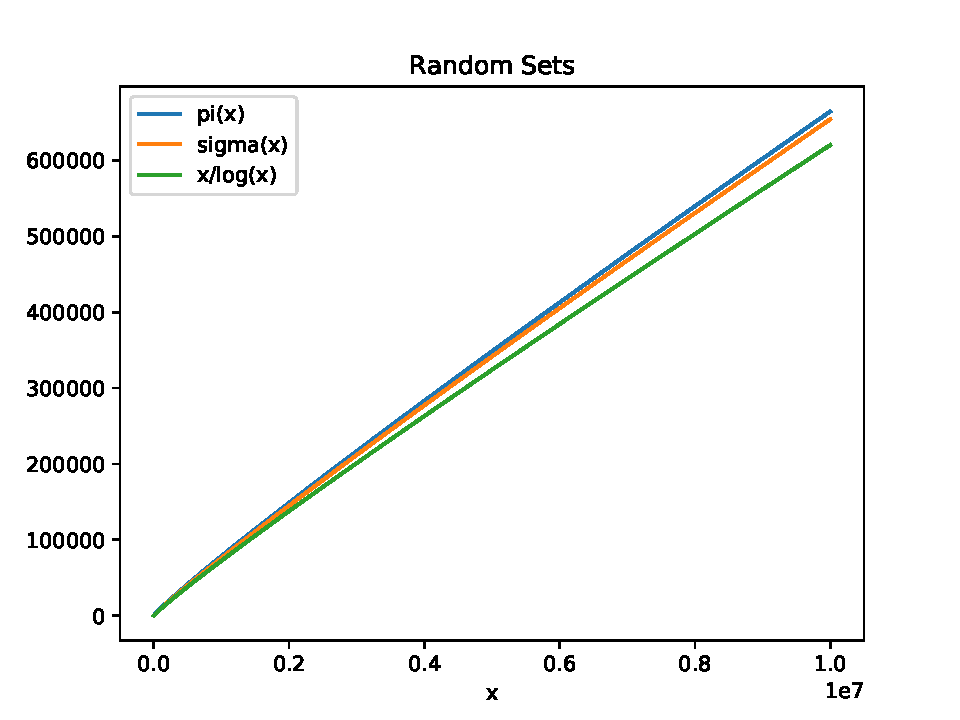
\includegraphics[keepaspectratio=true, width=12cm]{approche_analytique_sets.pdf}
 \caption{Graphe de $\sigma_{Q}$, $\pi$ et $\frac{x}{\log(x)}$ }
 \label{im:image1}
\end{figure}

\subsubsection{Écart entre $\pi(x)$ et $\sigma_{Q}(x)$}

La fonction $\sigma_{Q}$ semble suivre la même allure que $\pi$. Cependant, lors de nos expérimentations, nous avons dessiné des graphes (figures \ref{im:image2131}, \ref{im:image2132} et \ref{im:image2133}) pour des valeurs de $x$ inférieures à celles de la figure \ref{im:image1}. Pour des petites valeurs de $x$, la courbe de $\sigma_{Q}(x)$ était presque confondue avec celle de $\frac{x}{\log(x)}$. Lorsque les valeurs de $x$ sont de plus en plus grandes, $\sigma_{Q}(x)$ tend vers $\pi(x)$. Pour analyser l'écart entre $\pi(x)$ et $\sigma_{Q}(x)$, nous avons tracé le graphe de la fonction $ x \mapsto \frac{\pi(x)}{\sigma_{Q}(x)}$ : 

\begin{figure}[H]
 \centering
 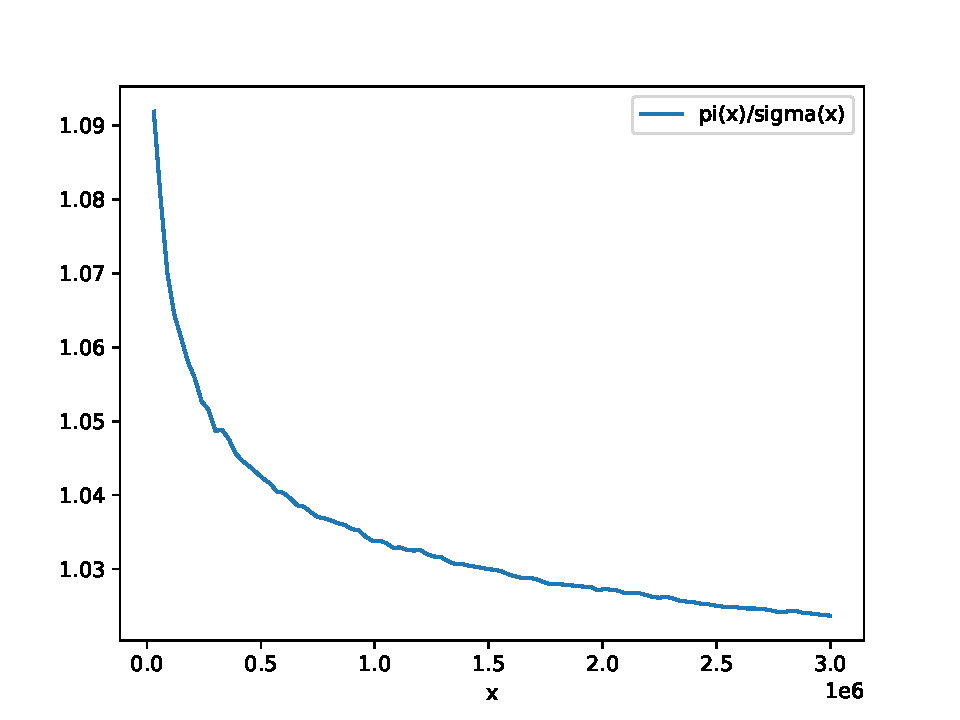
\includegraphics[keepaspectratio=true, width=12cm]{ecarts.pdf}
 \caption{Graphe de $\frac{\pi}{\sigma_{Q}}$ }
 \label{im:image2}
 \end{figure}
On peut supposer que $ \pi(x) \sim \sigma_{Q}(x) $.


\subsubsection{Le Théorème des Nombres Premiers}

L'objectif de cette section est de prouver la fidélité de nos ensembles aléatoires $Q$ à la répartition des nombres premiers en vérifiant si le théorème des nombres premiers (voir \ref{TNP}) est vrai quand on remplace $\pi(x)$ par $\sigma_{Q}(x)$. 
Pour démontrer le Théorème des Nombres Premiers, il a été démontré que, quand $x$ tend vers l'infini, Li($x$) $ \sim \frac{x}{\log(x)} $. Nous pouvons montrer, graphiquement, que lorsque $x$ tend vers l'infini, $ \sigma_{Q}(x) \sim $ Li($x$)  (voir figure \ref{im:image3}), ce qui implique que $ \sigma_{Q}(x) \sim \frac{x}{\log(x)} $.

\begin{figure}[H]
 \centering
 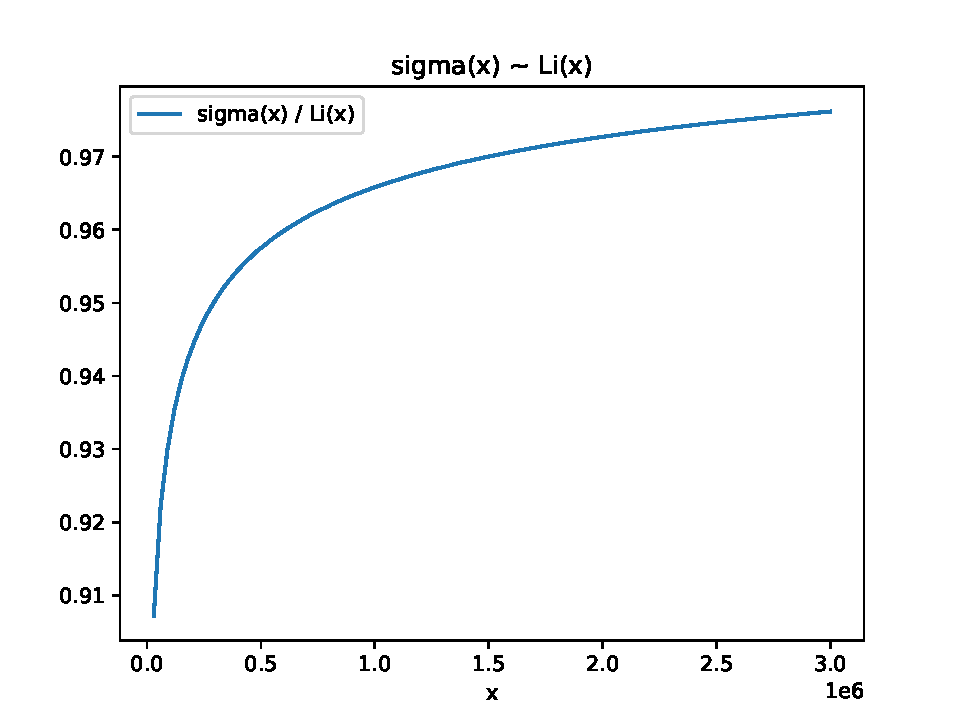
\includegraphics[keepaspectratio=true, width=12cm]{test2.pdf}
 \caption{Graphe de $\frac{\sigma_{q}}{Li}$}
 \label{im:image3}
 \end{figure}



\end{document}







